%!TEX root = ../../paper.tex
\begin{figure}
	\centering
	%!TEX root = ../../paper.tex

% Ferdosi 2, MBE
\begin{subfigure}{0.23\textwidth}
	\centering
	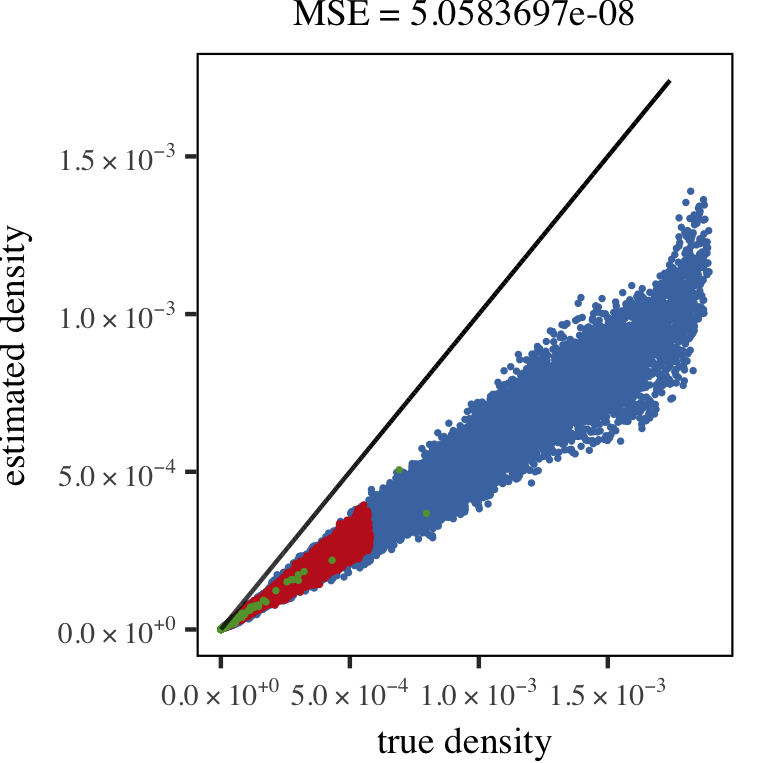
\includegraphics[keepaspectratio=true, width=\textwidth, height=0.23\textheight]{result/img/results_ferdosi_2_60000_mbe_silverman}
	\caption{Set \ferdosiTwo, \mbe}
	\label{fig:results:multisphere:mbe:ferdosi2}
\end{subfigure}
% Baakman 2, MBE
\begin{subfigure}{0.23\textwidth}
	\centering
	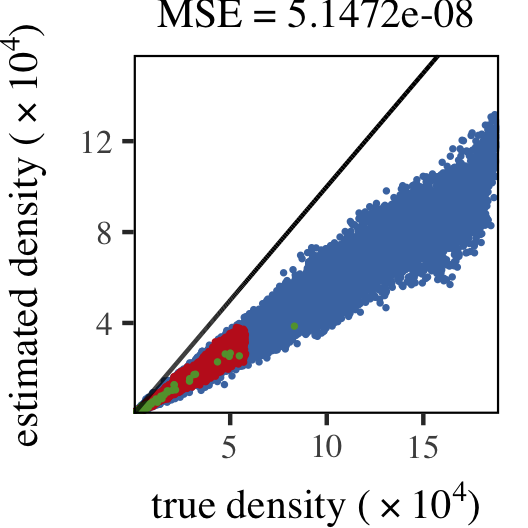
\includegraphics[keepaspectratio=true, width=\textwidth, height=0.23\textheight]{result/img/results_baakman_2_60000_mbe_silverman}
	\caption{Set \baakmanTwo, \mbe}
	\label{fig:results:multisphere:mbe:baakman2}
\end{subfigure}
% Ferdosi 2, SAMBE
\begin{subfigure}{0.23\textwidth}
	\centering
	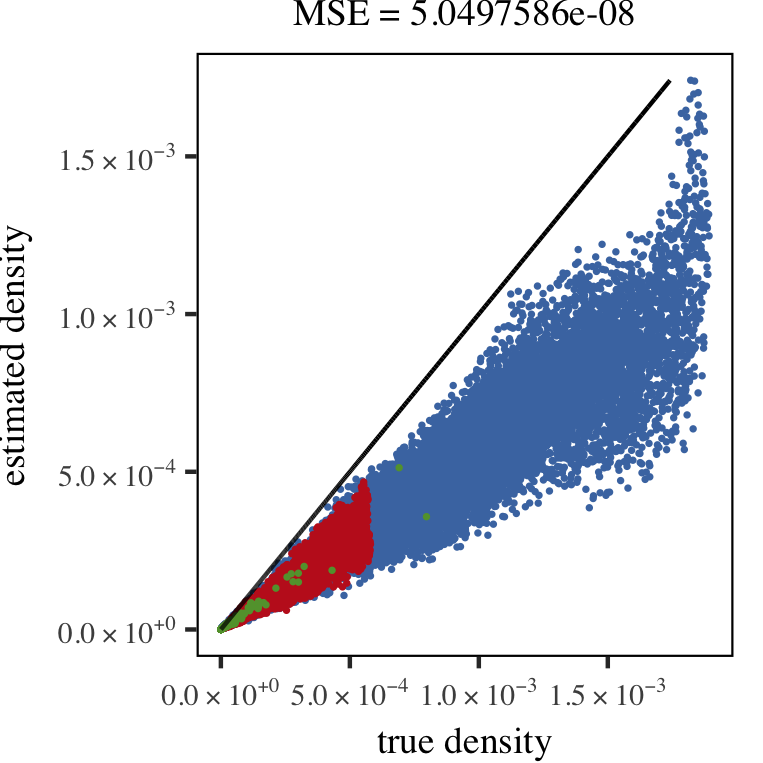
\includegraphics[keepaspectratio=true, width=\textwidth, height=0.23\textheight]{result/img/results_ferdosi_2_60000_sambe_silverman}
	\caption{Set \ferdosiTwo, \sambe}
	\label{fig:results:multisphere:sambe:ferdosi2}
\end{subfigure}
% Baakman 2, SAMBE
\begin{subfigure}{0.23\textwidth}
	\centering
	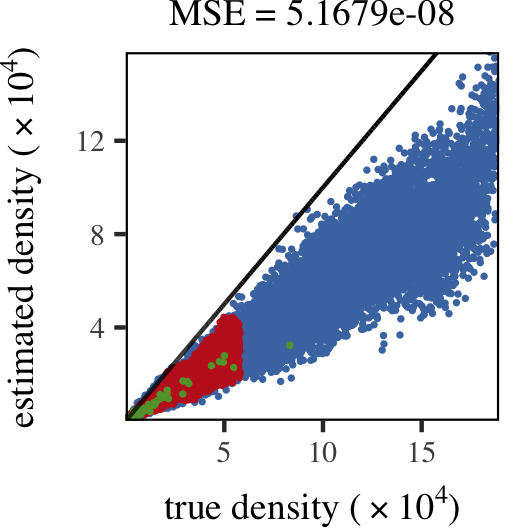
\includegraphics[keepaspectratio=true, width=\textwidth, height=0.23\textheight]{result/img/results_baakman_2_60000_sambe_silverman}
	\caption{Set \baakmanTwo, \sambe}
	\label{fig:results:multisphere:sambe:baakman2}
\end{subfigure}
	\caption{Plots of the true versus estimated density of datasets \ferdosiTwo and \baakmanTwo for the shape-adaptive and the symmetric Modified Breiman Estimator.}
	\label{fig:results:multiSphere:two:comparativePlots}
\end{figure}

\begin{figure}
	\centering
	%!TEX root = ../../paper.tex

% Ferdosi 3, MBE
\begin{subfigure}{0.33\textwidth}
	\centering
	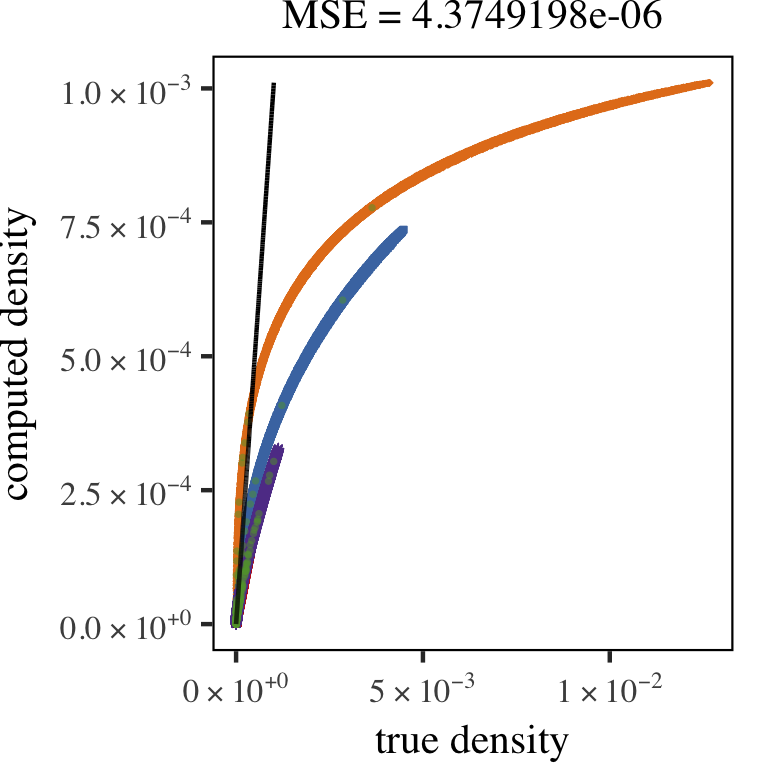
\includegraphics[keepaspectratio=true, width=\textwidth, height=0.23\textheight]{result/img/results_ferdosi_3_120000_mbe_silverman.png}
	\caption{Set \ferdosiThree, \mbe}
	\label{fig:results:multisphere:mbe:ferdosi3}
\end{subfigure}
% Baakman 3, MBE
\begin{subfigure}{0.33\textwidth}
	\centering
	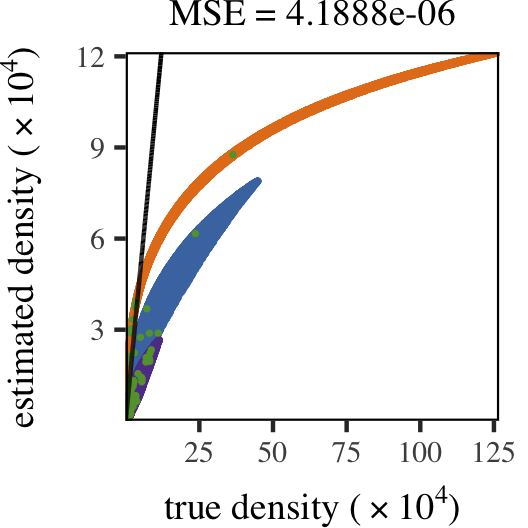
\includegraphics[keepaspectratio=true, width=\textwidth, height=0.23\textheight]{result/img/results_baakman_3_120000_mbe_silverman}
	\caption{Set \baakmanThree, \mbe}
	\label{fig:results:multisphere:mbe:baakman3}
\end{subfigure}	
% Ferdosi 3, SAMBE
\begin{subfigure}{0.33\textwidth}
	\centering
	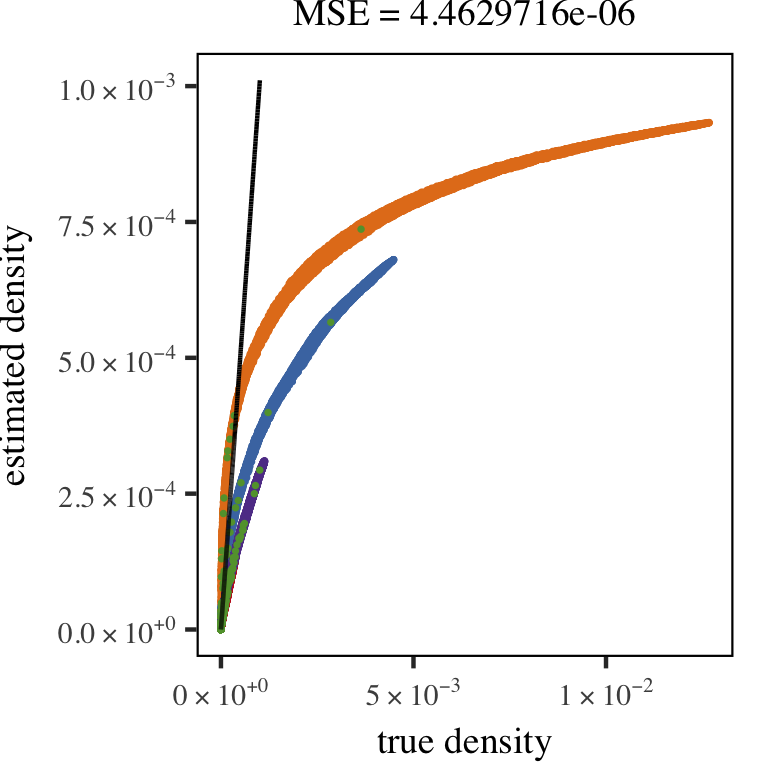
\includegraphics[keepaspectratio=true, width=\textwidth, height=0.23\textheight]{result/img/results_ferdosi_3_120000_sambe_silverman}
	\caption{Set \ferdosiThree, \sambe}
	\label{fig:results:multisphere:sambe:ferdosi3}
\end{subfigure}
% Baakman 3, SAMBE
\begin{subfigure}{0.33\textwidth}
	\centering
	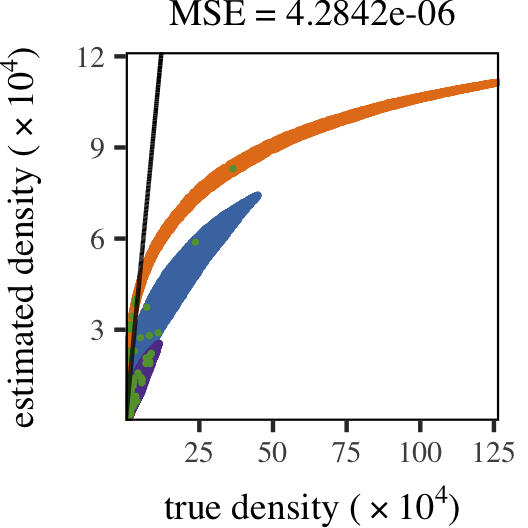
\includegraphics[keepaspectratio=true, width=\textwidth, height=0.23\textheight]{result/img/results_baakman_3_120000_sambe_silverman}
	\caption{Set \baakmanThree, \sambe}
	\label{fig:results:multisphere:sambe:baakman3}
\end{subfigure}	
	\caption{The estimated density plotted as a function of the true density for datasets \ferdosiThree and \baakmanThree for \mbe and \sambe.}
	\label{fig:results:multiSphere:three:comparativePlots}
\end{figure}

\begin{table}
	\centering
	%!TEX root = ../../paper.tex

\begin{tabular}{l*{2}{S[scientific-notation=true, round-mode=places,round-precision=3]}}
\toprule
~ 				& \multicolumn{2}{c}{Estimator}\\ \cmidrule{2-3}
Set				& {\mbe}					& {\sambe}	\\
\midrule
\ferdosiOne		& 8.30580618349064E-09		&  8.9087329457441E-09 \\
\baakmanOne		& 1.49022877061299E-08		&  1.5398737157543E-08 \\	
\baakmanFour	& 2.93709420107411E-08		&  2.9634323205557E-08 \\	
\baakmanFive	& 5.57179476550916E-08		&  5.5847473903432E-08 \\	
\bottomrule
\end{tabular}
	\caption{Performance of the symmetric and the shape-adaptive Modified Breiman Estimator on the datasets containing multiple Gaussian distributions.} 	
	\label{tab:results:multiSphere:mse}
\end{table}

\begin{table*}
	\centering
	%!TEX root = ../../paper.tex

% \sisetup{
% 	table-format=1.3e+1,
% 	scientific-notation=true, 
% 	table-number-alignment=center,
% }

% Mean and SD in single column
% \begin{tabular}{@{}c*{6}{c}@{}}
% \toprule
% ~				& Full Set 												& \legendComponentOne Gaussian 1						& \legendComponentTwo Gaussian 2						& \legendComponentThree Gaussian 3						& \legendComponentFour Gaussian 4					 	&  \legendComponentNoise Noise\\
% \midrule
% %
% \ferdosiTwo		& \meanSD{1.504005042371507e+00}{5.309582791641542e-01} & \meanSD{1.320121582169093e+00}{1.749869852989719e-01} & \meanSD{1.304784013773833e+00}{1.427734068384871e-01} & ~ 													& ~ 													& \meanSD{1.890276960903559e+00}{7.587403345342156e-01}\\
% \baakmanTwo 	& \meanSD{1.614716145373154e+00}{5.702499690627806e-01} & \meanSD{1.407377455694081e+00}{2.782480127488867e-01} & \meanSD{1.491043432778090e+00}{3.453168397321122e-01}	& ~ 													& ~ 													& \meanSD{11.948464282370670e+00}{7.826307984091438e-01}\\
% \ferdosiThree	& \meanSD{1.460357930082488e+00}{5.507084955708148e-01} & \meanSD{1.294023549845817e+00}{1.889517285607608e-01} & \meanSD{1.265946347671562e+00}{1.301150512342848e-01} & \meanSD{1.291829938425150e+00}{2.103396722315814e-01} & \meanSD{1.275739356043035e+00}{1.654855348814119e-01} & \meanSD{1.819950324176552e+00}{8.111641695146756e-01} \\
% \baakmanThree 	& \meanSD{1.532493079967588e+00}{5.713672219810757e-01} & \meanSD{1.314980484677339e+00}{2.190657831683435e-01} & \meanSD{1.487242917765238e+00}{3.393090417977690e-01} & \meanSD{1.291829938425150e+00}{2.103396722315814e-01} & \meanSD{1.396015162355687e+00}{2.851380764085146e-01} & \meanSD{1.854880861700560e+00}{8.195085323228068e-01}\\
% %
% \bottomrule
% \end{tabular}

\small
\sisetup{
	table-format=1.4,
	scientific-notation=fixed,
	table-number-alignment=center,
	fixed-exponent=0,
	round-mode=figures,
	round-precision=4
}


\begin{tabular}{@{}c*{12}{S}@{}}
\toprule
 				& \multicolumn{2}{c}{~} 						& \multicolumn{2}{c}{\legendComponentOne Gaussian 1} 	& \multicolumn{2}{c}{\legendComponentTwo Gaussian 2}	& \multicolumn{2}{c}{\legendComponentThree Gaussian 3}	& \multicolumn{2}{c}{\legendComponentFour Gaussian 4}	& \multicolumn{2}{c}{\legendComponentNoise Noise} \\
															  	\cmidrule(lr){4-5}							  				\cmidrule(lr){6-7}							  			\cmidrule(lr){8-9} 							  			\cmidrule(lr){10-11} 							  \cmidrule(lr){12-13}
~				& {\mean}				& {\SD}			& {\mean}				 & {\SD}			& {\mean}				 & {\SD}			 & {\mean}				& {\SD}			& {\mean}				& {\SD}			& {\mean}					& {\SD}\\ 			
\midrule
\ferdosiTwo		& 1.504005042371507e+00 & 5.309582791641542e-01 & 1.320121582169093e+00 & 1.749869852989719e-01 & 1.304784013773833e+00 & 1.427734068384871e-01 &  						&  						& 	 					&  							& 1.890276960903559e+00 	& 7.587403345342156e-01\\
\baakmanTwo 	& 1.614716145373154e+00 & 5.702499690627806e-01 & 1.407377455694081e+00 & 2.782480127488867e-01 & 1.491043432778090e+00 & 3.453168397321122e-01 &  						&  						& 	 					&  							& 1.948464282370670e+00 	& 7.826307984091438e-01\\
\ferdosiThree 	& 1.460357930082488e+00 & 5.507084955708148e-01 & 1.294023549845817e+00 & 1.889517285607608e-01 & 1.265946347671562e+00 & 1.301150512342848e-01 & 1.291829938425150e+00 & 2.103396722315814e-01 & 1.275739356043035e+00 & 1.654855348814119e-01 	& 1.819950324176552e+00 	& 8.111641695146756e-01 \\
\baakmanThree 	& 1.532493079967588e+00 & 5.713672219810757e-01 & 1.314980484677339e+00 & 2.190657831683435e-01 & 1.487242917765238e+00 & 3.393090417977690e-01 & 1.291829938425150e+00 & 2.103396722315814e-01 & 1.396015162355687e+00 & 2.851380764085146e-01 	& 1.854880861700560e+00 	& 8.195085323228068e-01\\
\bottomrule
\end{tabular}
	\caption{The mean and standard deviation of the anisotropy of the kernels used for points from the datasets with multiple Gaussians, split per component and for the full dataset.} 	
	\label{tab:results:multiSphere:anisotropy}
\end{table*}

% What does the section do
In this section we present the results of the two estimators on dataset \ferdosiTwo, \baakmanTwo, \ferdosiThree, and \baakmanThree.
% MSE
	% GENERAL
	Based on the small differences between the \mses of the estimators in \cref{tab:results:multiSphere:mse} the estimators perform comparably on these datasets. 
	% FERDOSI 2 
		% COMPONENT 1 MBE MSE 1.385919090205819e-07 SAMBE MSE 1.384478742850174e-07
		% COMPONENT 2 MBE MSE 1.313643043640668e-08 SAMBE MSE 1.302177563181053e-08
		% NOISE  	  MBE MSE 2.293851560028409e-11 SAMBE MSE 2.329767921658432e-11
	% BAAKMAN 2
		% COMPONENT 1 MBE MSE 1.407069060886291e-07 SAMBE MSE 1.412169246599802e-07
		% COMPONENT 2 MBE MSE 1.367299679831388e-08 SAMBE MSE 1.378034105739574e-08
		% NOISE 	  MBE MSE 3.497662493386784e-11 SAMBE MSE 3.920943401183576e-11	
	% FERDOSI 3	
		% COMPONENT 1 MBE MSE 2.390294620096452e-06 SAMBE MSE 2.466705633403533e-06
		% COMPONENT 2 MBE MSE 1.188881378312256e-08 SAMBE MSE 1.231201873705999e-08
		% COMPONENT 3 MBE MSE 2.373920131423336e-05 SAMBE MSE 2.418690791957957e-05
		% COMPONENT 4 MBE MSE 1.113882923683008e-07 SAMBE MSE 1.152633135516966e-07
		% NOISE 	  MBE MSE 4.320565280514733e-10 SAMBE MSE 4.461773022571117e-10
	% BAAKMAN 3
		% COMPONENT 1 MBE MSE 2.329212432941902e-06 SAMBE MSE 2.391586354071871e-06
		% COMPONENT 2 MBE MSE 1.748202359601445e-08 SAMBE MSE 1.764561034215026e-08
		% COMPONENT 3 MBE MSE 2.265532341806348e-05 SAMBE MSE 2.316257978616503e-05
		% COMPONENT 4 MBE MSE 1.312379885278773e-07 SAMBE MSE 1.339883658098755e-07
		% NOISE 	  MBE MSE 3.916881734521594e-10 SAMBE MSE 4.028048478164317e-10
	% FOCUS ON COMPONENTS
	Comparing the \MSE between components within the data sets between estimators yields no differences. However within data sets the difference in \mses are quite large.
	% FERDOSI 2 & BAAKMAN 2
	Within dataset \ferdosiTwo and \baakmanTwo both estimators perform significantly better on the more sparse component `Trivariate Gaussian 2'.
	% FERDOSI 3 & BAAKMAN 3
	Both estimators show the same positive correlation between the density of the Gaussian components and the \MSE between the components of dataset \ferdosiThree and \baakmanThree.


% PLOTS
	% GENERAL: TWO SPHERES
	\Cref{fig:results:multiSphere:two:comparativePlots} shows the estimated density as a function of the known density for both estimators and both datasets with two Gaussians. These plots show that both estimators underestimate the density, \mbe more than \sambe. Furthermore the shape-adaptive estimator shows more variation in the densities it estimates than the symmetric estimator. 
	% FERDOSI 2
	% BAAKMAN 2	
	% FOCUS ON COMPONENTS
	Comparing \cref{fig:results:multisphere:mbe:ferdosi2,fig:results:multisphere:mbe:baakman2} with \cref{fig:results:multisphere:sambe:ferdosi2,fig:results:multisphere:sambe:ferdosi2} suggest that \sambe hardly underestimates the densities of the most anisotropic component, \ie `Trivariate Gaussian 2' in bot dataset \ferdosiTwo and \baakmanTwo. However 

	% GENERAL: FOUR SPHERES

	% FERDOSI 3	

	% BAAKMAN 3

	% FOCUS ON COMPONENTS

% ANISOTROPY
	% GENERAL: TWO SPHERES

	% FERDOSI 2

	% BAAKMAN 2	

	% FOCUS ON COMPONENTS

	% GENERAL: FOUR SPHERES

	% FERDOSI 3	

	% BAAKMAN 3

	% FOCUS ON COMPONENTS

% SUMMAR/CONCLUSION
	%GENERAL - SOMETHING ON THE HYPOTHESES

	%FOCUS ON COMPONENTS





\oldStuff

%Introduction
	In this section we present the results of the two estimators on dataset \ferdosiTwo, \baakmanTwo, \ferdosiThree, \baakmanThree.

% Ferdosi 2
	% General difference
	Comparing \cref{fig:results:multisphere:mbe:ferdosi2} with \cref{fig:results:multisphere:sambe:ferdosi2} we find that both estimators underestimate the density and that the densities estimated by the \sambe are spread out more than those estimated by \mbe. In spite of this the difference in \mse between the two estimators is small enough to be insignificant. 
	% Components
	The same holds for the \mse of the individual components.

% Baakman 2
	% General difference
	\Cref{fig:results:multisphere:mbe:baakman2,fig:results:multisphere:sambe:baakman2} show the same general trend as \cref{fig:results:multisphere:mbe:ferdosi2,fig:results:multisphere:sambe:ferdosi2}: both estimators underestimate, the shape-adaptive estimator less so than the symmetric estimator, but the differences between the two estimators are small. 
	% Components
	The differences in \MSE within the difference components between the estimators are negligible. 
	% Contrast to Ferdosi 2
	Comparing the performance of the estimators between datasets \ferdosiTwo and \baakmanTwo we find that the performance of both estimators hardly suffers from the elongation of the Gaussians. 

% Ferdosi 3
	% General Differnence
	\Cref{fig:results:multisphere:mbe:ferdosi3,fig:results:multisphere:sambe:ferdosi3} clearly show that both estimators significantly underestimate the true density, \sambe more so than \mbe. 
	% Components
	Comparing the \mse of the different components we find that both estimators performed worst on the densest component, and best on the component with the highest value on the diagonal of its covariance. There is no significant difference between the estimators within the different components. 

% Baakman 3
	% General Difference
	\Cref{fig:results:multisphere:mbe:baakman3,fig:results:multisphere:sambe:baakman3} shows the same underestimating of densities as the plot of the plots associated with datasets \ferdosiThree. Compared to densities estimated for that dataset the range of densities estimated by both estimators for dataset \baakmanThree is greater. The difference in \mse within both the complete set and 
	% Components
	its components between the two estimators is negligible. 
	% Constrast to Ferdosi 3
	Contrary to our expectations both estimators perform better on the elongated dataset, \ie \ferdosiThree, than on the spherical set. 

% General
	In general we have found that the number of Gaussian distributions embed in the noise negatively influences the performance of both estimators. Furthermore the denser a Gaussian distribution is, the more difficulty the estimators have with correctly approximating the density of the points sampled from it. 